\documentclass[12pt]{report}
\usepackage[margin=1in]{geometry}
\usepackage{setspace} % for single/doublespacing commands
\usepackage{graphicx} % including graphics
\usepackage{sectsty} % sexy section headings
\usepackage{pdfpages} % including multipage pdfs
\usepackage[export]{adjustbox} % for graphic frames and center
\usepackage{siunitx}
\usepackage[numbered]{matlab-prettifier} % including matlab w/ syntax highlighting
\usepackage[T1]{fontenc} % prettier matlab font
\usepackage{xfrac} % more legible inline fractions (\sfrac)
\usepackage{lmodern} % font package for above
\usepackage{multicol} % multiple columns
\usepackage[justification=centering]{caption} % figure captions (force centering)
\usepackage{amsmath} % more math symbols and shit
\usepackage{enumitem} % add arguments for enumerate to change style
\usepackage[list=true]{subcaption} % subfigures with list of figure support
\usepackage{multirow}
\usepackage{mathtools}
\usepackage{booktabs}
\usepackage{color}
\usepackage{ulem}
\usepackage{blindtext}
\usepackage{natbib}
\usepackage{contour}
\usepackage{tabularx}
\usepackage{circuitikz} % drawing fancy shit
\usepackage{cancel} % arrow and cross math cancel symbol
\usepackage{lineno}
\usepackage{framed}
\usepackage{amssymb} % special math symbols
\usepackage{listings}
\usepackage{array}
\usepackage{BOONDOX-cal} % fancy mathtype script
\usepackage{fancyhdr}
\usepackage{flowchart}

\setcounter{secnumdepth}{5}
\renewcommand{\bibname}{References}
\sisetup{output-exponent-marker=\ensuremath{\mathrm{e}}}
\newcommand{\PreserveBackslash}[1]{\let\temp=\\#1\let\\=\temp}
\newcolumntype{C}[1]{>{\PreserveBackslash\centering}p{#1}}
\newcolumntype{R}[1]{>{\PreserveBackslash\raggedleft}p{#1}}
\newcolumntype{L}[1]{>{\PreserveBackslash\raggedright}p{#1}}
\lstMakeShortInline[style=Matlab-editor]| % matlab inline escape character
\graphicspath{{images/}}
\renewcommand\thesection{\arabic{section}}
\renewcommand\labelitemi{---}
\lstset{numberstyle=\ttfamily\small\color{gray}}
\renewcommand\linenumberfont{\ttfamily\small\color{gray}}
\setlength\linenumbersep{6mm}
% \hbadness=99999  % or any number >=10000
\usetikzlibrary{arrows,calc,patterns,angles,quotes}
\usetikzlibrary{shapes.geometric}
\usetikzlibrary{decorations.pathmorphing,decorations.pathreplacing} % for snakes!
\usetikzlibrary{positioning, circuits.logic.US}
% Define block styles
\tikzstyle{decision} = [diamond, draw, fill=white!20,
    text width=4.5em, text badly centered, node distance=3cm, inner sep=0pt]
\tikzstyle{term} = [rectangle, draw, fill=white!20,
    text width=5em, text centered, rounded corners, minimum height=2em]
\tikzstyle{block} = [rectangle, draw, fill=white!20,
    text width=4em, text centered, minimum height=4em]
\tikzstyle{line} = [draw, -latex']
\tikzstyle{cloud} = [draw, ellipse,fill=white!20, node distance=3cm,
    minimum height=2em]
\tikzstyle{data} = [trapezium,trapezium left angle=70,
    trapezium right angle=-70,draw, minimum height=1cm]
\tikzstyle{proc} = [draw, predproc, align=center,
    minimum width=4em, minimum height=1cm]

\newcommand{\Lag}{\mathcal{L}} % lagrangian L

\begin{document}
\normalem
\begin{titlepage}
\flushleft
\doublespacing
\Large
\textsc{Test Document} \\
\normalsize
Trey Dufrene, Zack Johnson, David Orcutt, Alan Wallingford, Ryan Warner
\vfill
\center
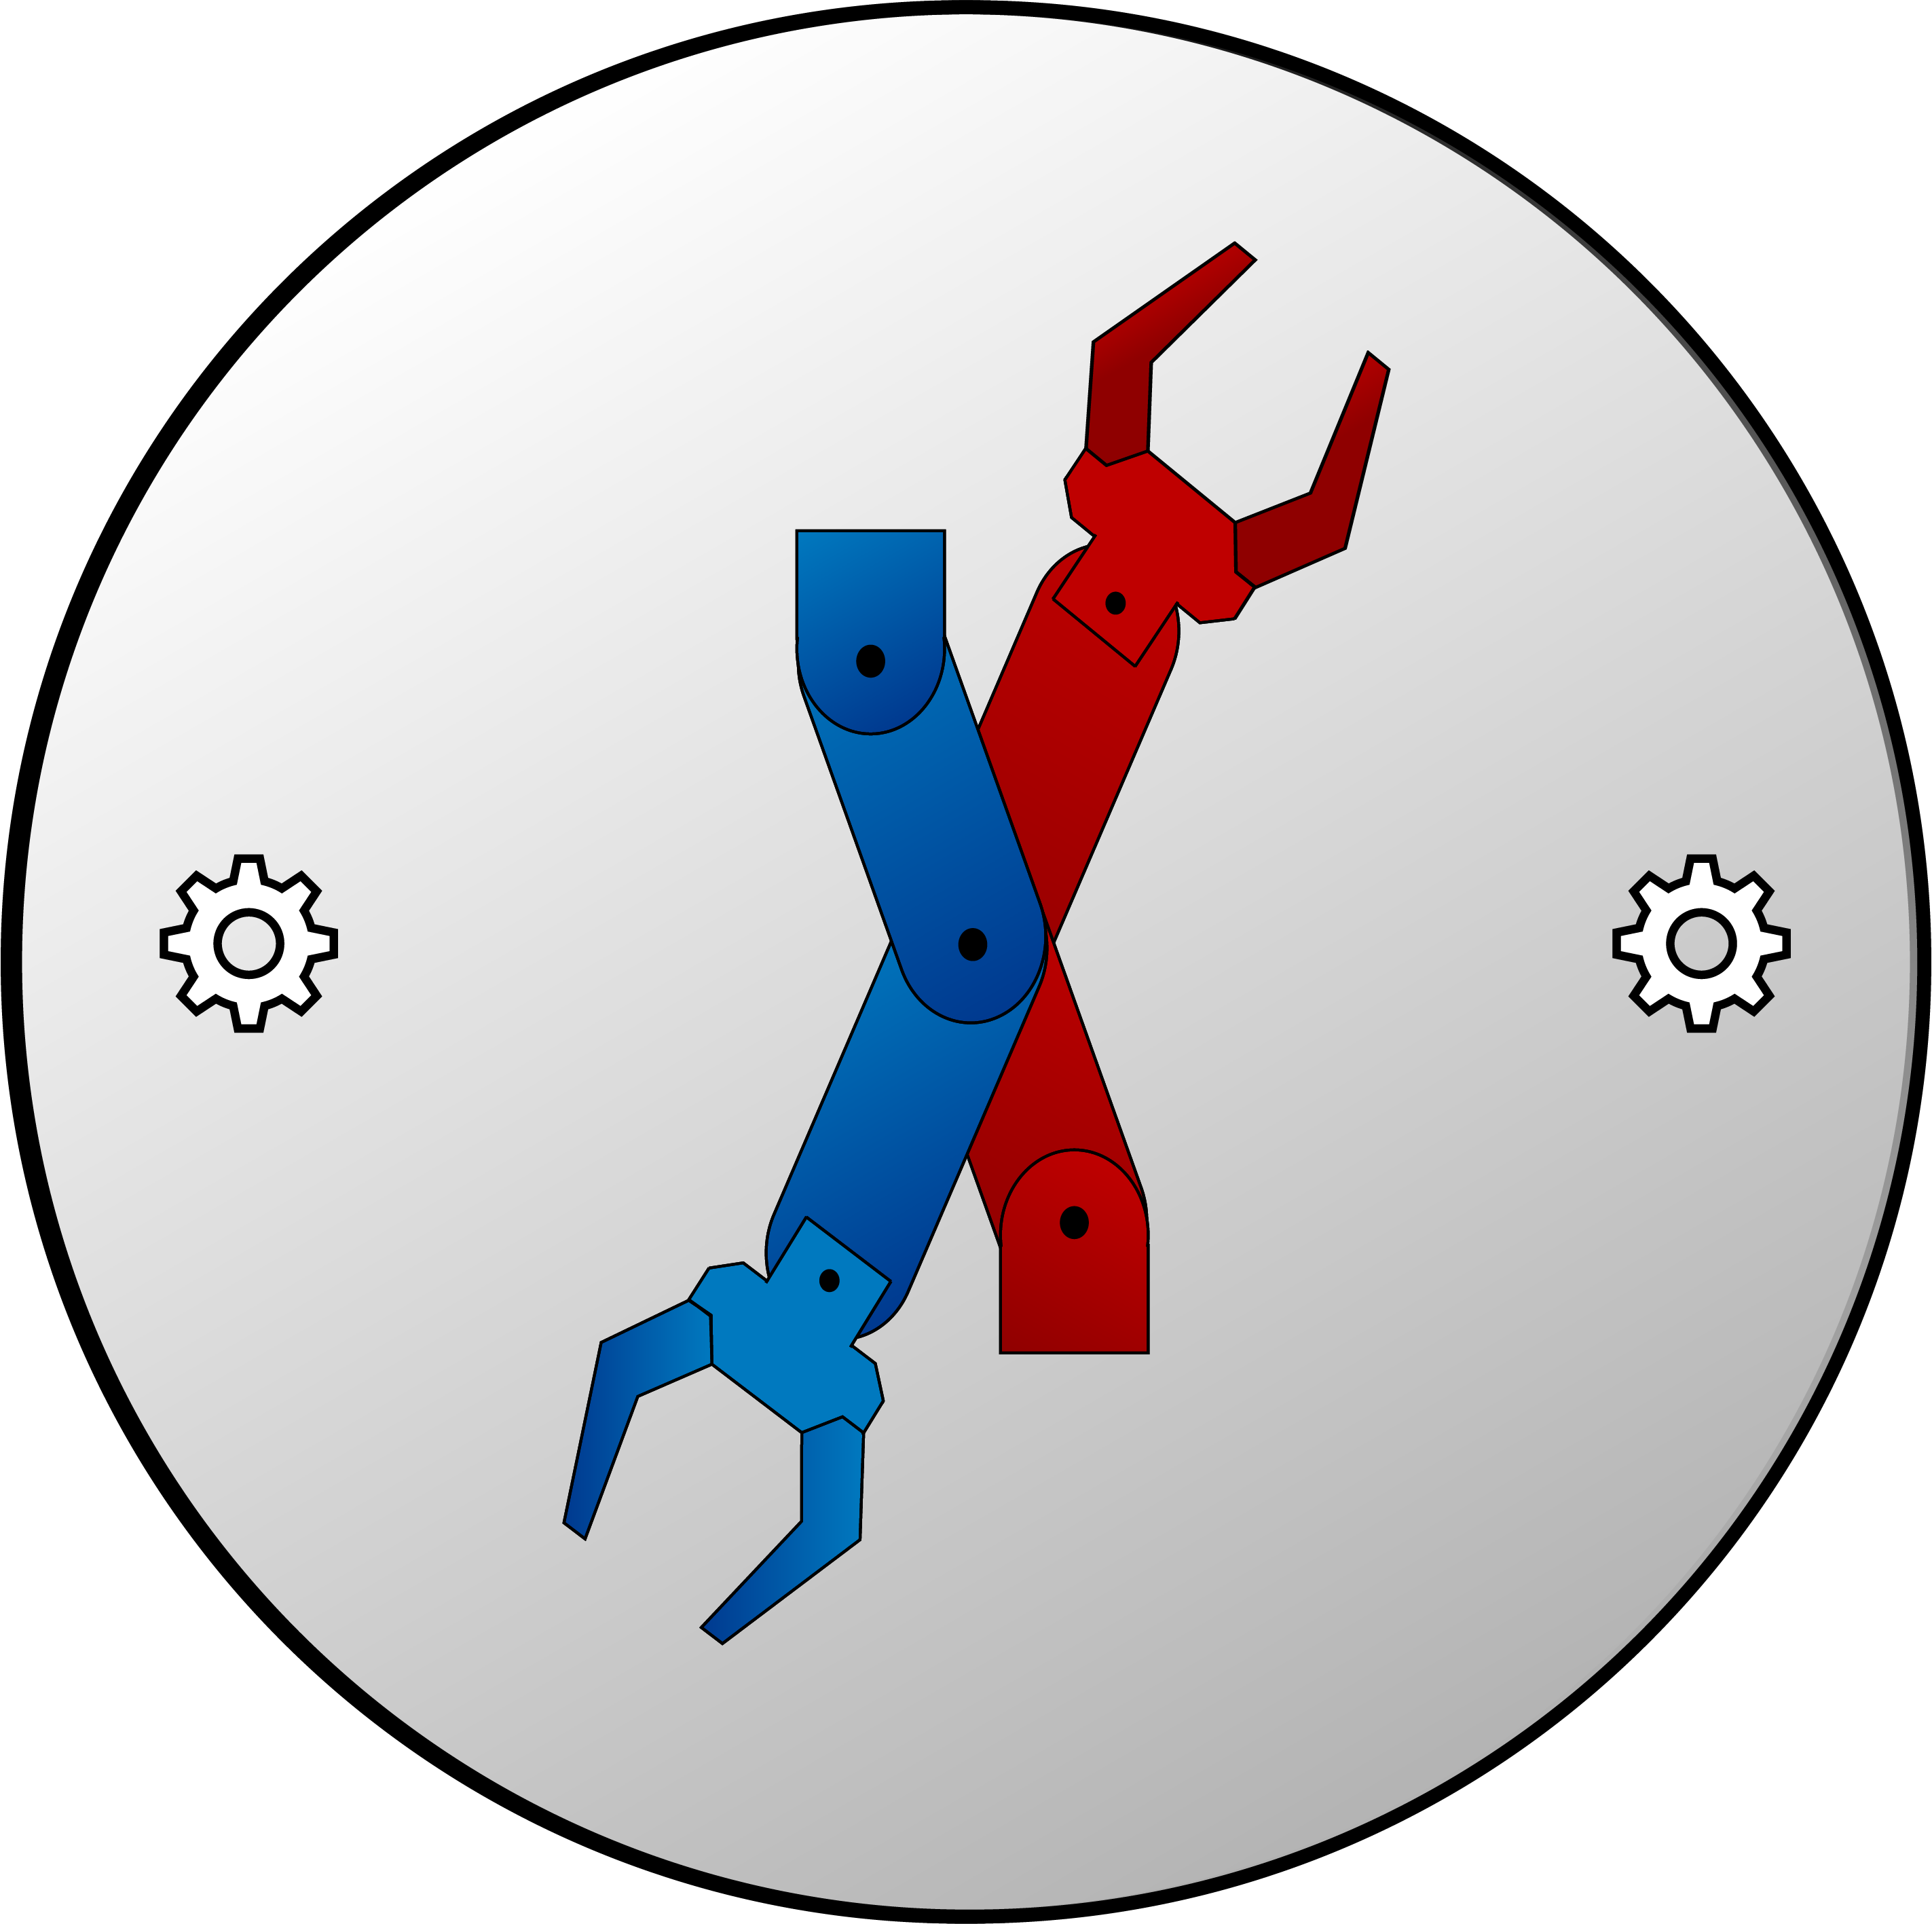
\includegraphics[width=.45\textwidth]{logo}
\vfill
\flushleft
ME 407 \\
Preliminary Design of Robotic Systems \\
Embry-Riddle Aeronautical University \\
\vspace{2ex}
\begin{minipage}[c]{.5\textwidth}
\flushleft

\includegraphics[width=.95\textwidth]{erau}
\end{minipage}%
\begin{minipage}[c]{.5\textwidth}
\flushright

\includegraphics[width=.8\textwidth]{text}
\end{minipage}
\end{titlepage}

\pagenumbering{roman}
% \begin{abstract}
  % Wordy words
% \end{abstract}
{\tableofcontents\let\clearpage\relax\listoffigures\let\clearpage\relax\listoftables}
\clearpage
\newpage

% \section*{List Of Acronyms and Abbreviations}

% \begin{tabular}{rl}
%   $G$~:&Center of gravity of the bar \\
%   $\ell_0$~:& Spring unstretched length  \\
%   $\delta$~:& Spring deflection \\
%   $k$~:& Spring constant \\
%   $h_{b}$~:& Distance to bar ($G$) from datum \\
%   $F_s$~:& Force onto bar due to spring\\
%   $A_{n}$~:& Pin reaction in $\theta$ direction\\
%   $A_{t}$~:& Pin reaction in tangential direction \\
%   $\vec{v}_G$~:& Velocity of bar center of gravity\\
%   $\ddot{\theta}$~:& Angular velocity of spring \\
%   $\ddot{\phi}$~:& Angular velocity of bar\\
%   $\ddot{\ell}_s$~:& Radial acceleration of spring \\
% \end{tabular}
% \normalsize
% \flushleft
% \singlespacing
% \newpage

\pagenumbering{arabic}
\onehalfspacing
\section{Introduction}
The terminator T-2000 is a science-fiction spectacle of a manipulator-- until you see the price. Channeling the inspiration many high school students may have for robotics, MEIOSIS robotics aims to provide an affordable manipulator to educators and enthusiasts. MEIOSIS uses primarily 3-D printed components and easily accessible materials. Among these materials are a Raspberry PI , smart servos and metal tubing. These features create an open-source manipulator accessible to the public to further robotics education.
\section{Physical System Overview}
\emph{Figure \ref{fig:overall}} shows the overall design for the manipulator. Much of the system’s physical design will be determined during the actual design of the manipulator, after the specifications stage. The figure below shows the basic overall conceptual design of the manipulator, having all six rotational joints, the latter three of which being in a spherical wrist configuration.

\begin{figure}[h]
  \centering
  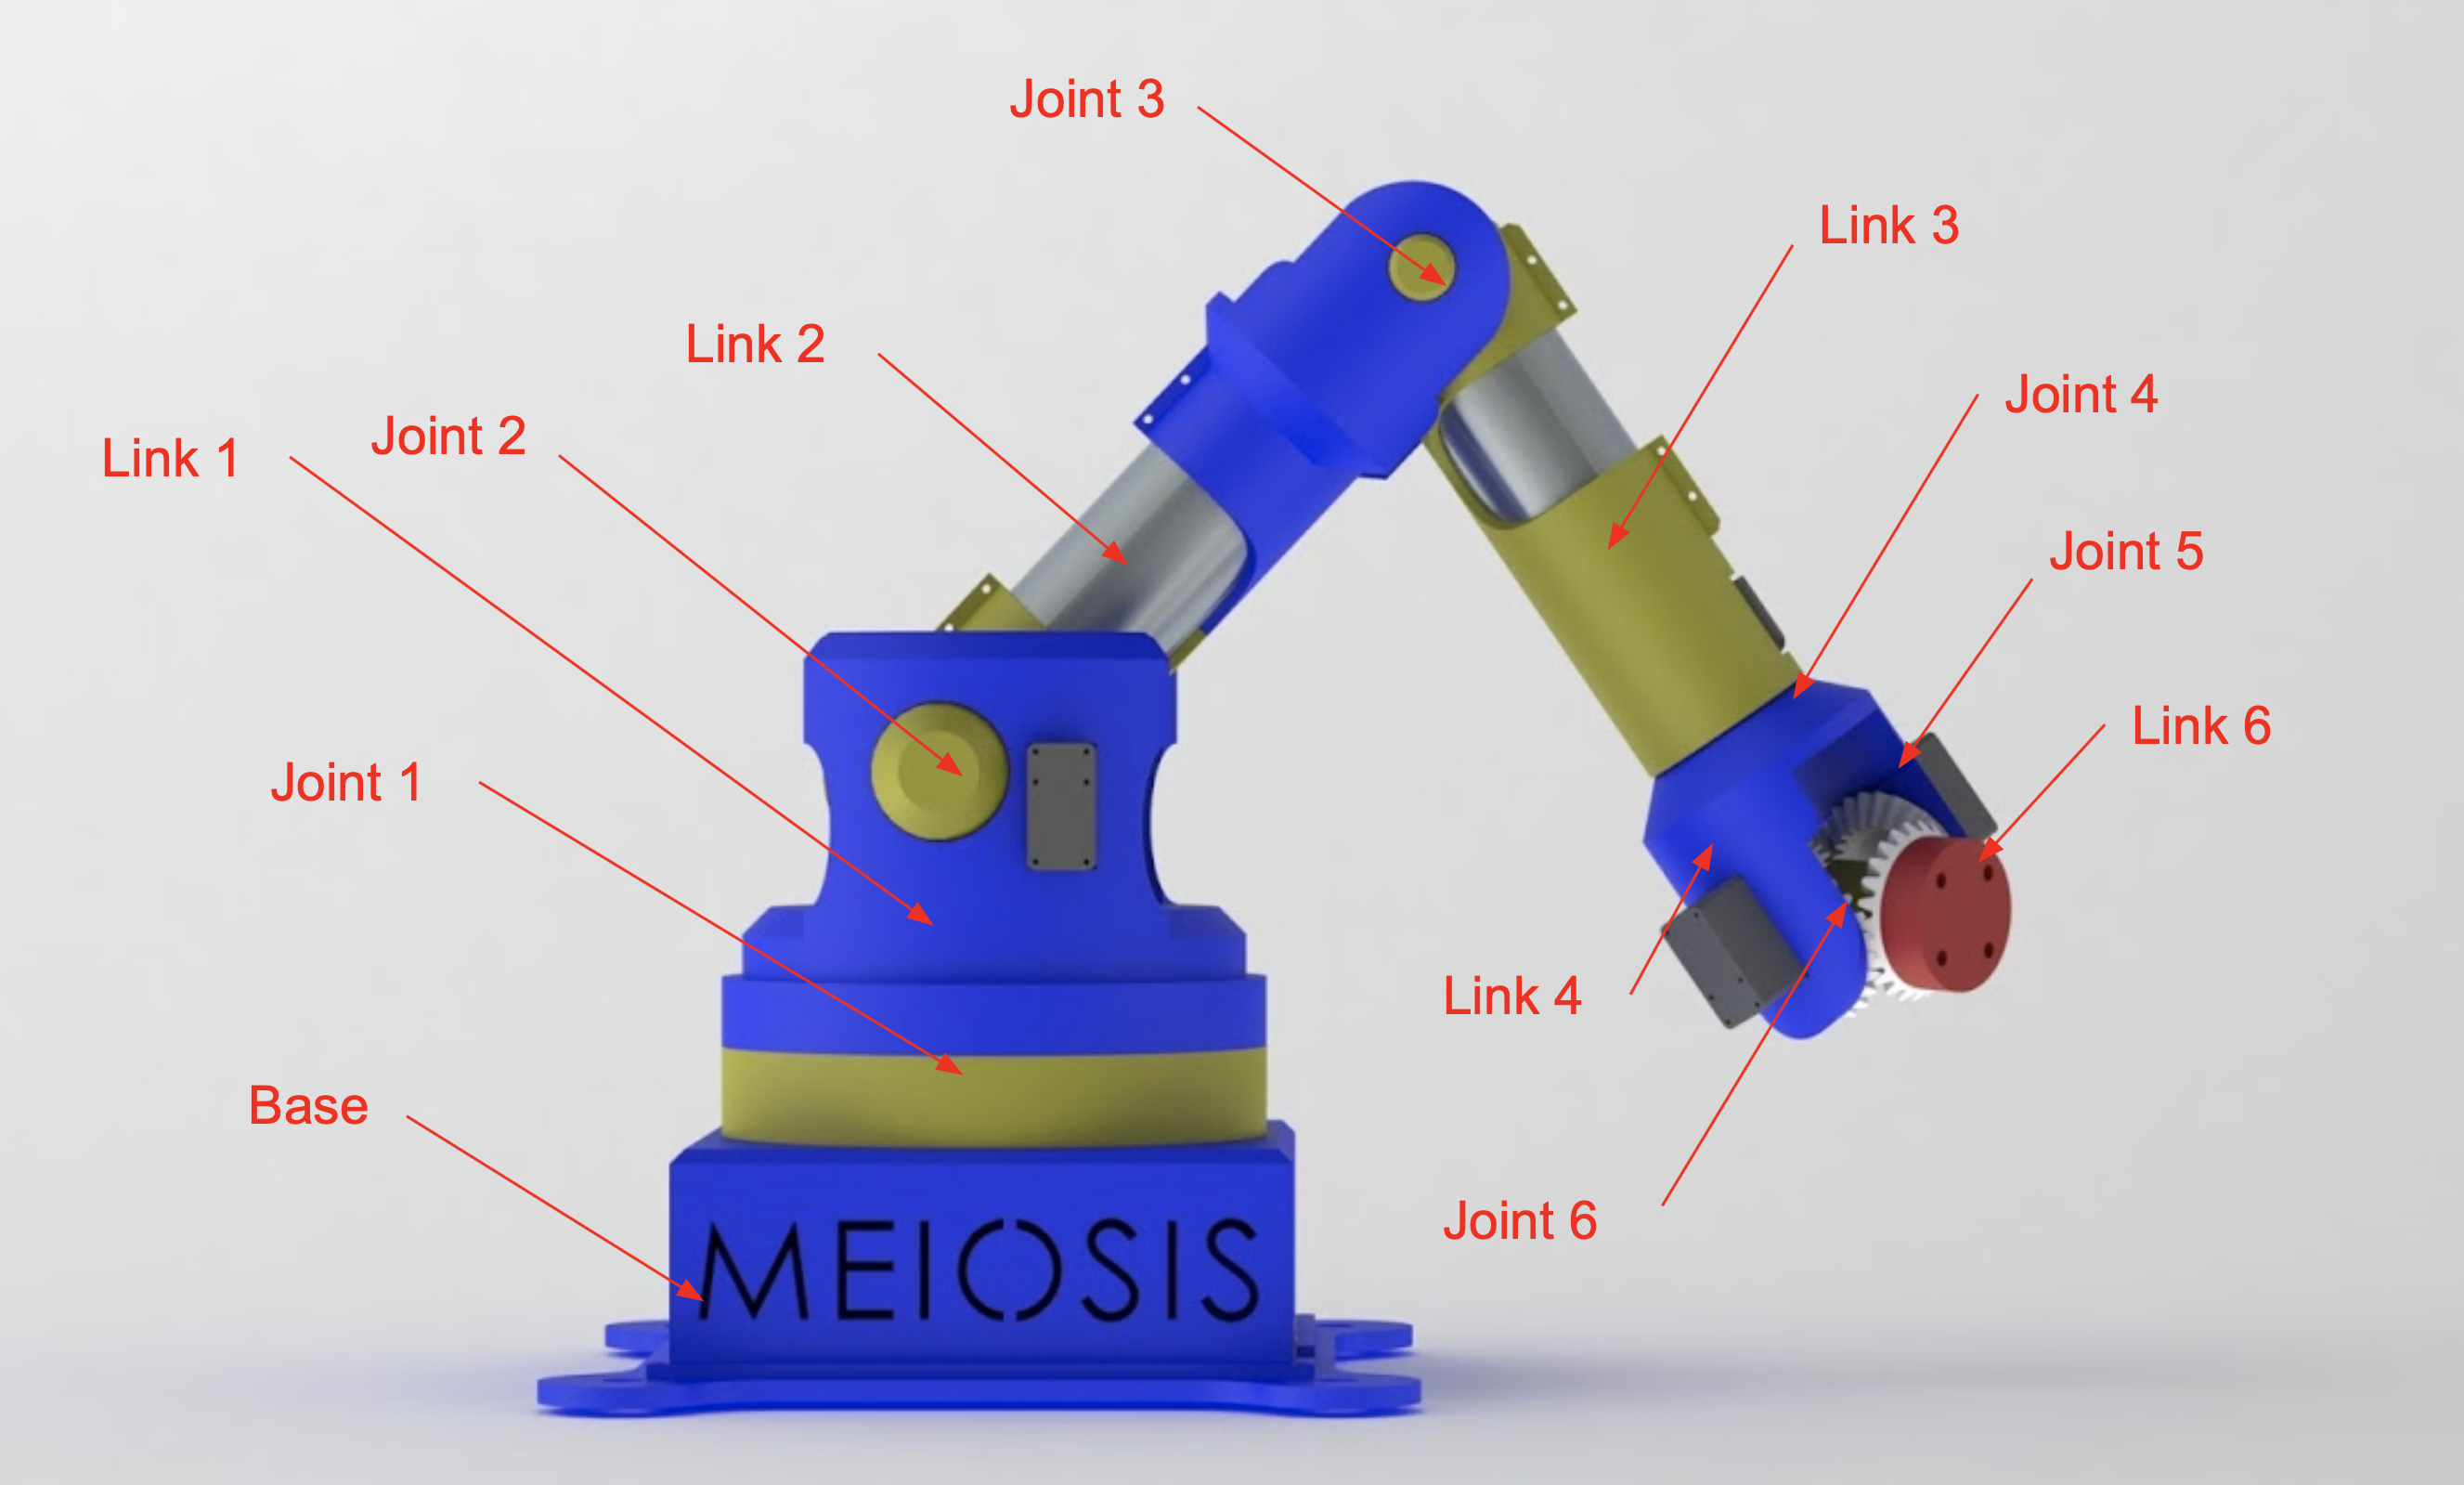
\includegraphics[frame, width=.75\textwidth]{overall_render}
  \caption{Overall System Conceptual Design }
  \label{fig:overall}
\end{figure}

The colored links in \emph{Figure \ref{fig:overall}} distinguish the different joints and links of the manipulator. The overall reach of the robot will be 500 mm. This length was chosen to decrease material cost and weight while still satisfying requirement 2.1.2 and 2.1.5, allowing the manipulating to pick and place objects to perform basic tasks. The base of the robot will be made to contain the Raspberry Pi and other electrical components.
\newpage
\subsection{Base}
The base of the manipulator will house several of the electronic components, such as the computational sytem, power supply, and motor controller. A cross section of the base can be seen in \emph{Figure \ref{fig:base}}.
\begin{figure}[h]
  \centering
  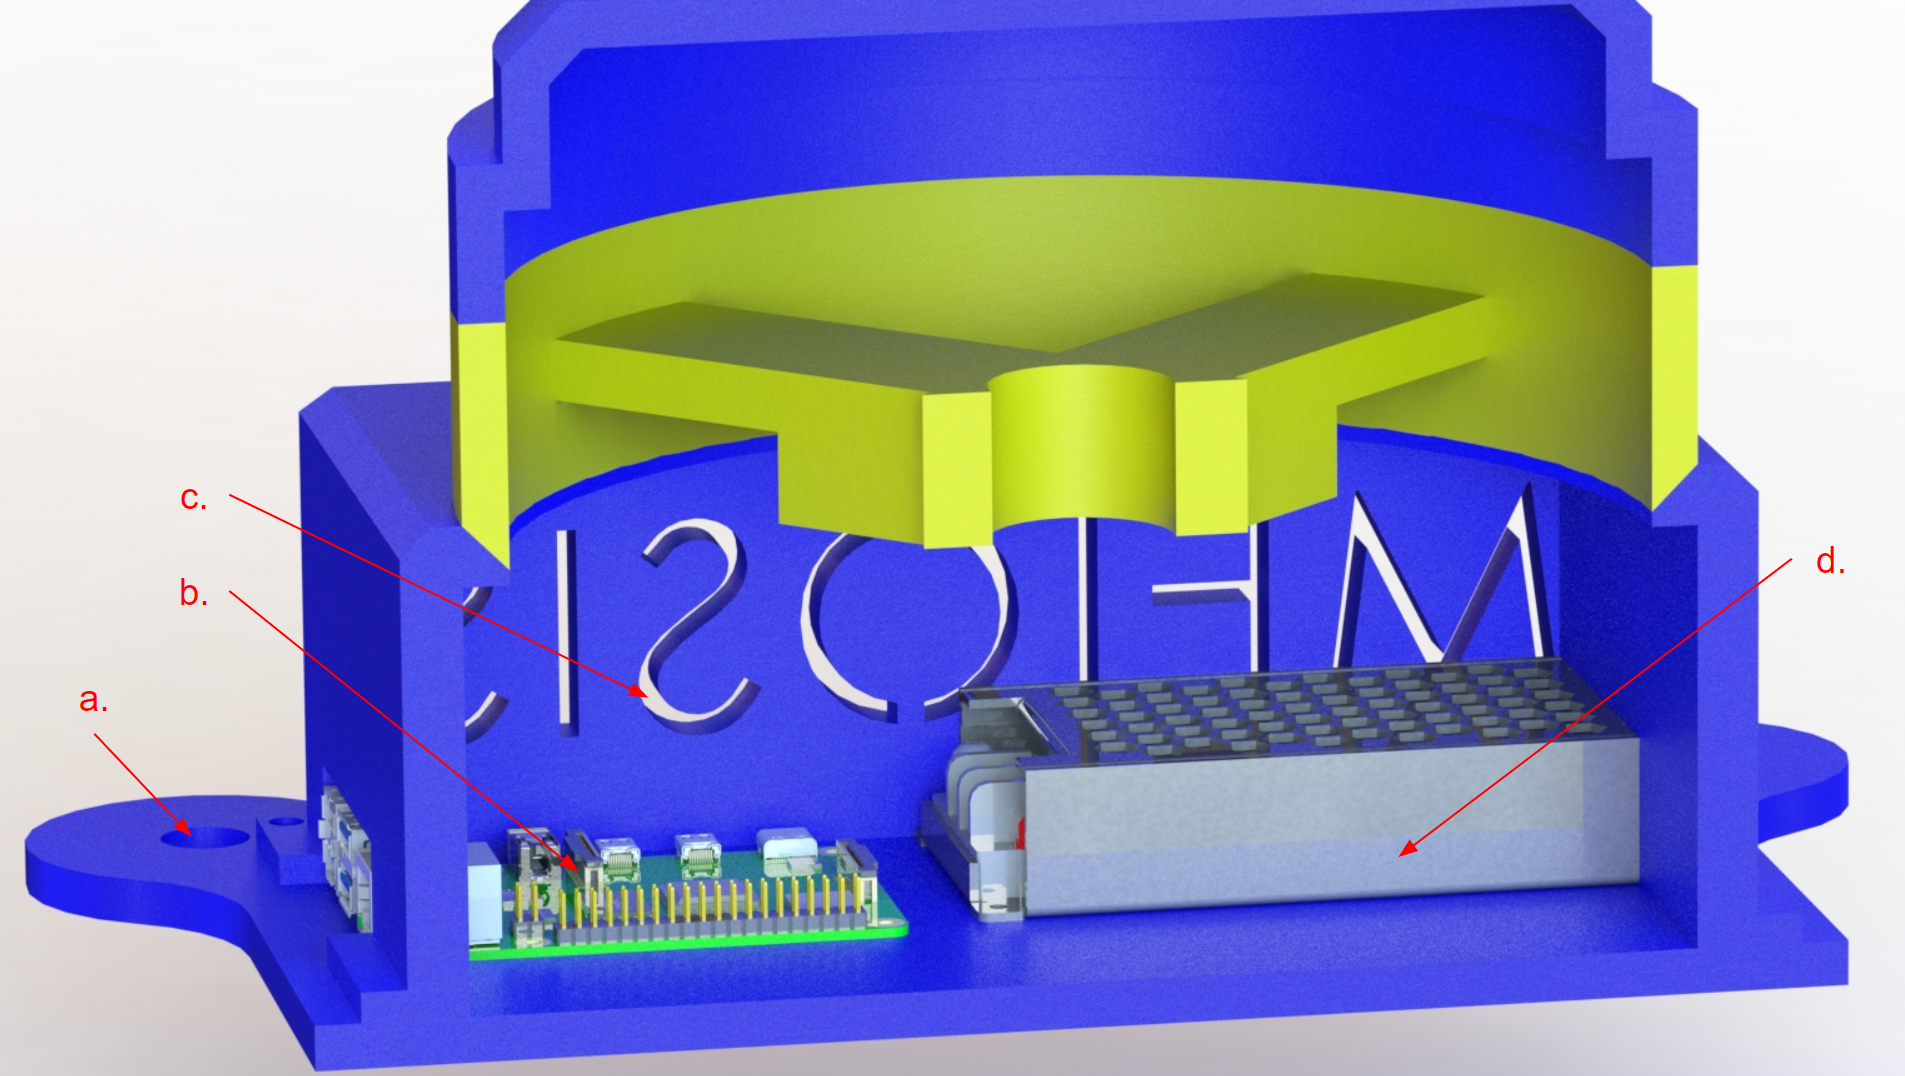
\includegraphics[frame, width=.75\textwidth]{base_callouts}
  \caption{Manipulator Base with Callouts}
  \label{fig:base}
\end{figure}

From \emph{Figure \ref{fig:base}},
\begin{enumerate}[label=\alph*.]
  \item \emph{Base Supports:}
  The base supports are located at each corner of the base and will allow the base of the manipulator to be securely attached to a variety of surfaces with either standard bolt/fastener hardware or suction cups.
  \item \emph{Computational System:}
  The computational system will consist of a Raspberry Pi; the primary reason for this system being chosen is to fulfill the budget requirement, 2.1.1. The Raspberry Pi will perform the necessary computations for solving the kinematics of the manipulator and command the motors accordingly.
  \item \emph{Airflow Cutouts:}
  The side of the base will have cutouts to allow for the maximum amount of airflow to pass through; since the power supply is housed inside of the base as well as the computational system, the temperature must be regulated to prevent overheating.
  \item \emph{Power Supply:}
  The power supply will be housed in the base as well; this allows the system to be more accessible and therefore more modifiable, where the end-user can easily expand the system to fulfill their needs.
\end{enumerate}
%
% \subsection{Joints 1 \& 2}
% Much of the system’s physical design will be determined during the actual design of the manipulator, after the specifications stage. The figure below shows the basic overall conceptual design of the manipulator, having all six rotational joints, the latter three of which being in a spherical wrist configuration.
\newpage

\section{System Functions}
The system consists of two primary categories, the electrical and software systems. The electrical subsystem includes the wiring and hardware computational components, power system, actuators with drivers, and sensors. The software subsystem includes the algorithm flowchart for the computational system as well as the intended end-user interface platform. 
\subsection{Electrical System}

\begin{figure}[h]
  \centering
  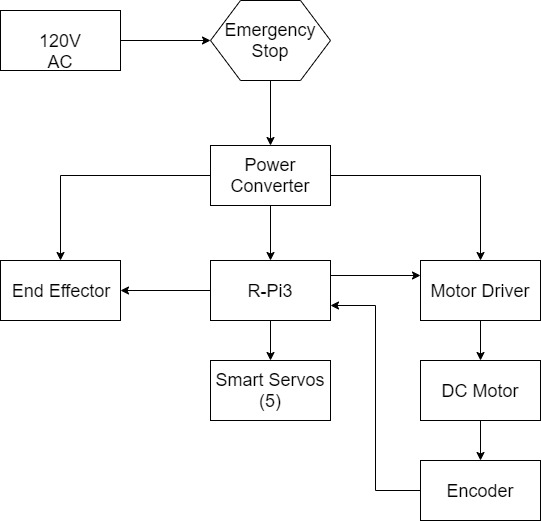
\includegraphics[width=.75\textwidth]{eblock}
  \caption{Electrical System Block Diagram}
  \label{fig:eblock}
\end{figure}

\emph{Figure \ref{fig:eblock}} shows that the electrical systems of the manipulator will be relatively simple, with power being supplied by the standard 120V AC available from wall outlets. A power converter will be used to adapt the AC voltage to the required voltages for each component. To control the system, a Raspberry Pi will perform the necessary calculations for motor control (described below in software). It will then send these signals to the DC motor driver and the five smart servos. The smart servos have an on-board controller, so no feedback will be necessary. However, the first rotational joint between the base and the first link will be actuated by a DC motor with an encoder to minimize cost.


% \center
% \null\vspace{20ex}
% \begin{tikzpicture}
%   \draw (-1cm,0) -- (0,0) coordinate (base);
%   \draw (0,0) -- (1cm,0);
%   \draw (-1cm,-.5cm) -- (-1cm,0);
%   \draw (1cm,-.5cm) -- (1cm,0);
%   \node[cylinder, draw, rotate=90, label=1,
%   minimum height=1.5cm, minimum width=1cm] at (0,1.5cm) (1) {};
%   \draw (base) -- (1);
%
%
% \end{tikzpicture}

% \section{Electrical System}
% The electrical-mechanical overview is shown below
% \subsection{Electrical System Flowchart}
%
% \begin{figure}[ht]
%   \centering
%   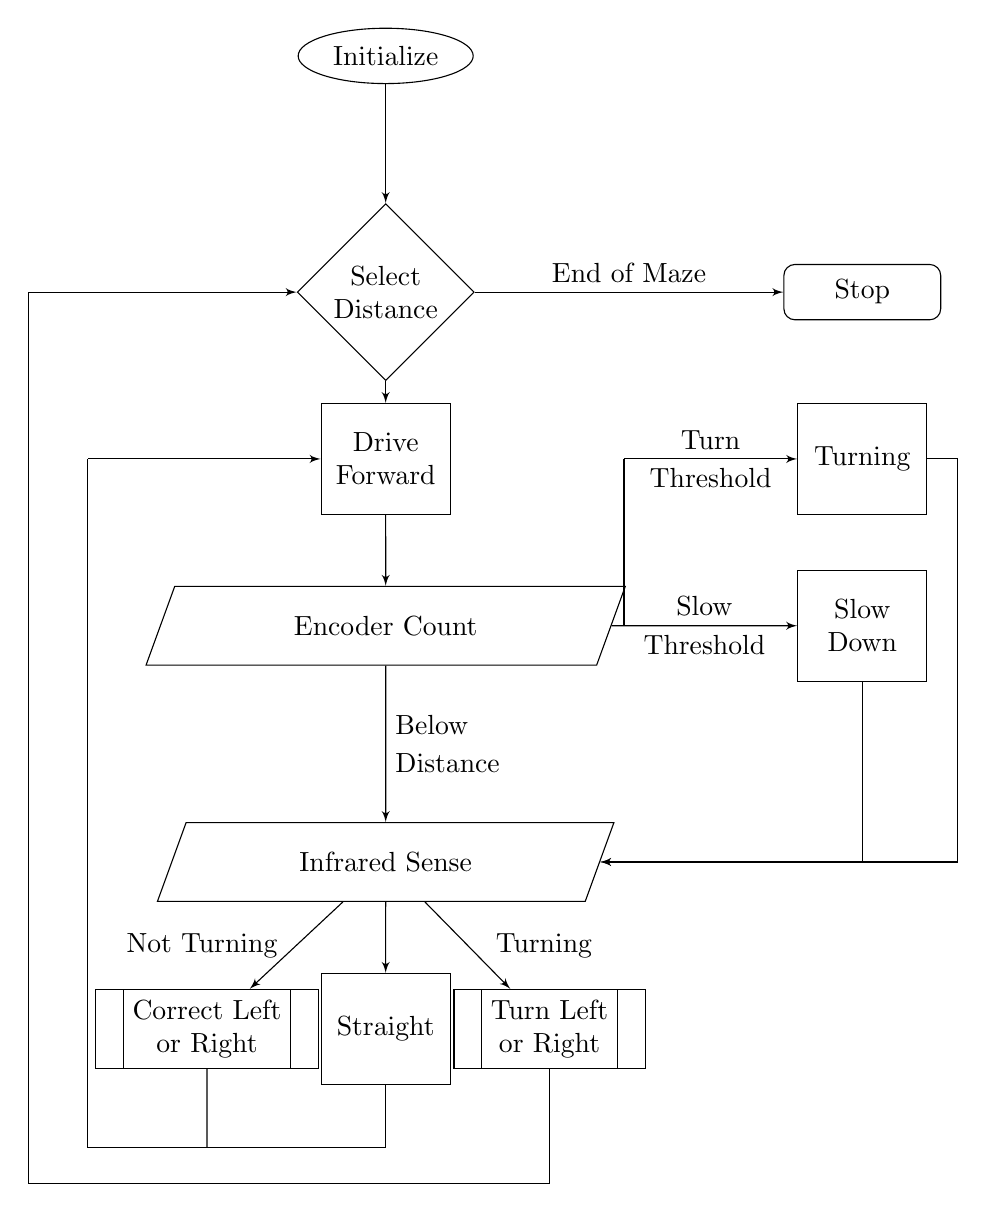
\begin{tikzpicture}[node distance = 14ex, auto]
    \node [cloud] (init) {Initialize};
    \node [decision, below of=init] (select) {Select Distance};
    \node [block, below of=select] (drive) {Drive Forward};
    \node [data, below of=drive] (encoder) {Encoder Count};
    \node [data, below of=encoder, node distance=3cm] (ir) {Infrared Sense};
    \node [block, below of=ir] (straight) {Straight};
    \node [proc, left of=straight,node distance=15ex] (correct) {Correct Left \\ or Right};
    \node [block, right of=encoder,node distance=40ex] (slow) {Slow Down};
    \node [block, right of=drive,node distance=40ex] (stop) {Turning};
    \coordinate [below of=correct,node distance=10ex] (pathtodrive) {};
    \coordinate [left of=drive,node distance=25ex] (pathtodrive2) {};
    \coordinate [right of=drive,node distance=20ex] (pathtoturning) {};
    \coordinate [right of=stop,node distance=8ex] (pathtoturn) {};
    \node [proc,right of=straight,node distance=13.75ex] (turn) {Turn Left\\ or Right};
    \node [term, right of=select, node distance=40ex] (end) {Stop};
    \coordinate [below of=straight,node distance=13ex] (pathtoselect) {};
    \coordinate [left of=correct,node distance=15ex] (pathtoselect2) {};

    \path [line] (init) -- (select);
    \path [line] (select) -- (drive);
    \path [line] (drive) -- (encoder);
    \path [line] (encoder) -- node [above right]{Below} node[below right]{Distance}(ir);
    \path [line] (encoder) -- node[below]{Threshold} node[above]{Slow} (slow);
    \path [line] (ir) -- node[left]{Not Turning~~}(correct);
    \path [line,-] (correct) -- (pathtodrive);
    \path [line] (ir) -- (straight);
    \path [line,-] (encoder) -| (pathtoturning);
    \path [line] (pathtoturning) -- node [above]{Turn} node[below]{Threshold} (stop);
    \draw [line,-] (straight) |- (pathtodrive) -| (pathtodrive2);
    \path [line] (slow) |- (ir);
    \path [line] (stop) -- (pathtoturn) |- (ir);
    \path [line] (ir) -- node[right]{~~Turning} (turn);
    \path [line] (turn) |- (pathtoselect) -| (pathtoselect2) |- (select);
    \path [line] (pathtodrive2) -- (drive);
    \path [line] (select) -- node [above]{End of Maze} (end);
\end{tikzpicture}

%   \caption{Flow}
%   % \label{fig:overall}
% \end{figure}



% Example citations:
% \cite{DBLP:journals/corr/JohnsonAL16}
% \cite{DBLP:journals/corr/abs-1803-09820}
% \cite{DBLP:journals/corr/RonnebergerFB15}

% \section{A Level Heading}
% Sample table with tabulated data and reference label
% \begin{table}[htp]
%   \center
%   \caption{DH Table for 6 DOF Manipulator}
%   \label{table:dh}
%   \color{red} bold col headers, table times new roman, 12pt., centered, \color{black} \\
%   \begin{tabular}{C{1cm}|C{1cm}C{2cm}C{1cm}C{1cm}}
%     \textbf{DH} & $d_i$ & $\theta_i$ & $a_i$ & $\alpha_i$ \\ \hline
%     1 & 280 & $q_1 - \pi$ & 0 & $\sfrac{\pi}{2}$ \\
%     2 & 0 & $q_2 + \sfrac{\pi}{2}$ & 210 & 0 \\
%     3 & 0 & $q_3 - \sfrac{\pi}{2}$ & 75 & -$\sfrac{\pi}{2}$ \\
%     4 & 210 & $q_4$ & 0 & $\sfrac{\pi}{2}$ \\
%     5 & 0 & $q_5 - \pi$ & 0 & $\sfrac{\pi}{2}$ \\
%     6 & 70 & $q_6$ & 0 & 0 \\
%   \end{tabular}
% \end{table}
% here is the table reference callout
% \emph{Table \ref{table:dh}} shows the Denavit–Hartenberg parameters for the manipulator.

% Here is a centered mathtype with no number
% $$
% \vec{v}_G =
% \left[\dot{\ell}_s\sin(\theta) + \frac{\ell_b\dot{\phi}\cos(\phi)}{2} +
% \ell_s\dot{\theta}\cos(\theta)\right]\hat{\textrm{\i}} +
% \left[\frac{\ell_b\dot{\phi}\sin(\phi)}{2} -
% \dot{\ell}_s\cos(\theta) + \ell_s\dot{\theta}\sin(\theta)\right]\hat{\textrm{\j}}
% $$

% Here is a centered equation with number and reference label
% \begin{equation}
% \ddot{\theta} = \frac{d}{dt}\left(\frac{\partial\Lag}{\partial\dot{\theta}}\right) -
% \frac{\partial\Lag}{\partial\theta} = \big(Q_{\theta}\big)_{\text{non}}
% \label{eq:lagtheta}
% \end{equation}

% This is some inline mathtype: $u = \frac{1}{2}mv^2$, (notice the fluidity and smaller size than the other mathtype)

% \section{A Level Heading}
% \begin{figure}[h]
%   \centering
%   \includegraphics[width=.75\textwidth]{filename}
%   \caption{Figure with Callouts}
%   \label{fig:figname}
% \end{figure}

% \begin{enumerate}[label=\alph*.]
%   \item Description for callout a
%   \item Description for callout b
% \end{enumerate}

% As seen in \emph{Figure \ref{fig:figname}}

% \newpage
% \bibliographystyle{plain}
% \bibliography{JohnsonAL16,abs-1803-09820,RonnebergerFB15}

% \newpage
% \section*{Acknowledgements \& Attributions}
% \begin{itemize}
%   \item People!
% \end{itemize}
% \newpage

% \newpage
% \appendix
% \renewcommand\thesection{\Roman{section}}
% \renewcommand\thesubsection{\roman{subsection}}
% \section*{Appendix}\label{sec:app}
% Code listing
%\begin{lstlisting}[frame=lines,style=Matlab-editor,basicstyle = \mlttfamily, caption=Example Code
% Code Here
%\end{lstlisting}

% \includepdf[landscape,pages=-]{pdfname}

\end{document}
